
\section{Comparison of Coastal and Inland climates}
For the task not listed in the project description, a comparison is chosen. The idea is to compare the measurements of Visby, located on the small island of Gotland, to another set of measurements taken at an inland location. The produced histogram should thus highlight the differences of the two locations.

One way in which the temperature of coastal regions differs from those more inland is that the temperature changes overall more slowly. This is due to the large body of water acting as either a massive heat reservoir in the autumn of taking large amounts of energy to heat up in spring. Thus, one way to compare the locations would be to plot the temperatures in these transitional months of the year and see the temperature difference.

The second location is chosen to be Boras. It is chosen as it is of approximately the same altitude as Visby and is not a coastal city.

\subsection{Code structure}
To achieve this, the first step is to read the data. The method used is the \textbf{getline()} command, that saves the important data to strings which are then converted to integers and doubles. Before this, in order to make the data in the .csv file more manageable, a bash script is called with the \textbf{system()} function. The goal is to trim away all unnecessary text and only leave measurements of green quality marking.

This is all done in a while-loop, which can also be used to extract the temperatures of desired dates. As the only distinction needed for this comparison is to pick out measurements originating from a chosen month, a simple if-statement separates these from unwanted ones. A small script inside the statement calculates the temperature average for each day. These averages are then added to the histograms. To demonstrate more clearly the differences in temperature between the locations each histogram is fitted to a Gaussian function.

\subsection{Results}
When plotting the results of the comparison in May month, figure \ref{May} is created. As is easily seen, Boras tends to have higher temperatures than Visby during this period. While this coincides with the hypothesis, it alone does not prove it. 

\begin{figure}
	\centering
	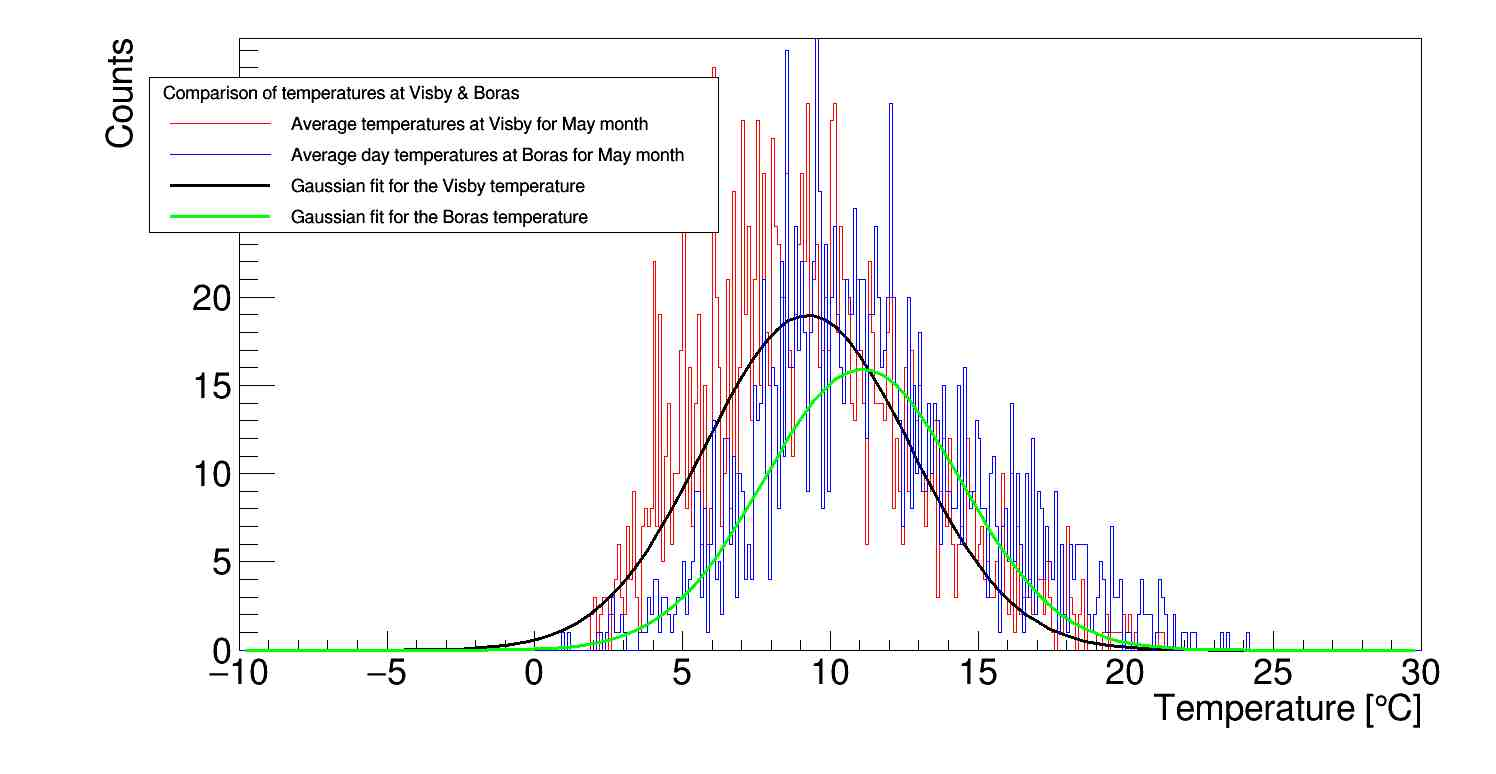
\includegraphics[width=14cm]{VisbyMay.jpg}
	\caption{Comparison between the Visby and Boras temperatures in May}
	\label{May}
\end{figure}

To further strengthen the hypothesis the temperature difference in autumn must also be investigated. In figure \ref{Sept} the temperatures for the two locations in September are shown.

Here, as predicted, Boras has the lower temperature. The water retains the heat of summer, causing Visby to decrease in temperature more slowly than for inland locations.  

\begin{figure}
	\centering
	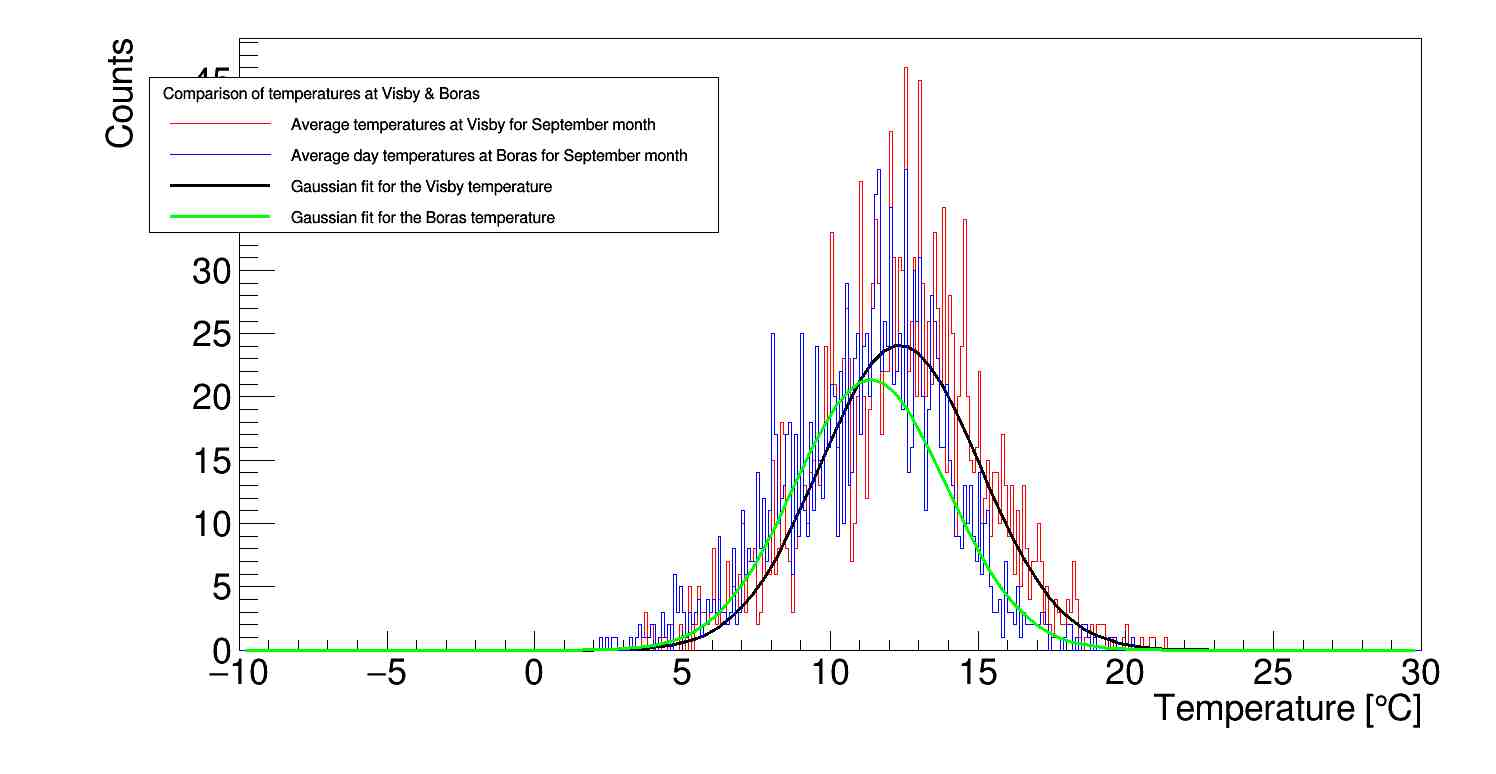
\includegraphics[width=14cm]{VisbySeptember.jpg}
	\caption{Comparison between the Visby and Boras temperatures in September}
	\label{Sept}
\end{figure}
